\documentclass{article}

% Bibliography
\usepackage{natbib}
\bibpunct{(}{)}{;}{a}{}{;}

% Use 'It was found that A is B (Name 1234)' style
\setcitestyle{authoryear,open={},close={}}

% Affiliations
\usepackage{authblk}
\title{
  Transmembrane helices are also 
  an overlooked source of major histocompatibility complex class II epitopes
  and evolutionary more conserved than expected by chance
}
\author[1]{Rich\`el J.C. Bilderbeek}
\author[2]{Frans Bianchi}
\affil[1]{Groningen Institute for Evolutionary Life Sciences, University of 
Groningen, Groningen, The Netherlands}
\affil[2]{Frans' Institute, University of Groningen, Groningen, The Netherlands}

% Use double spacing
\usepackage{setspace}
\doublespacing

\usepackage{listings}
\usepackage{hyperref}
\usepackage{todonotes}
\usepackage{verbatim}
\usepackage{pgf}
\usepackage{bm}
\usepackage{multirow}
\usepackage{amsfonts}
\usepackage{array}
\usepackage{array}
\usepackage{booktabs}
\newcolumntype{C}[1]{>{\centering\arraybackslash}p{#1}}
\newcolumntype{L}[1]{>{\raggedright\arraybackslash}p{#1}}
\usepackage{longtable}

\usepackage{tkz-graph}
\usetikzlibrary{arrows,automata}
\usetikzlibrary{calc}
\usetikzlibrary{arrows.meta}

% sidewaysfigure
\usepackage{rotating}

% Style of listings
% From http://r.789695.n4.nabble.com/
%   How-to-nicely-display-R-code-with-the-LaTeX-package-listings-tp4648110.html
\usepackage{fancyvrb} 
\definecolor{codegreen}{rgb}{0,0.6,0}
\definecolor{codegray}{rgb}{0.5,0.5,0.5}
\definecolor{codepurple}{rgb}{0.58,0,0.82}
\definecolor{backcolor}{rgb}{0.95,0.95,0.92}
\lstdefinestyle{mystyle}{
  language=R,% set programming language
  basicstyle=\ttfamily\small,% basic font style
  commentstyle=\color{gray},% comment style
  numberstyle=\scriptsize,% use small line numbers
  numbersep=10pt,% space between line numbers and code
  tabsize=2,% sizes of tabs
  showstringspaces=false,
  captionpos=b,% positioning of the caption below
  breaklines=true,% automatic line breaking
  escapeinside={(*}{*)},% escaping to LaTeX
  fancyvrb=true,% verbatim code is typset by listings
  extendedchars=false,% prohibit extended chars (chars of codes 128--255)
  alsoletter={.<-},% becomes a letter
  alsoother={$},% becomes other
  otherkeywords={!=, ~, $, \&, \%/\%, \%*\%, \%\%, <-, <<-, /},
  deletekeywords={c}% remove keywords 
}
\lstset{style=mystyle}

% Adds numbered lines. Not yet...
% \usepackage{lineno}
% \linenumbers

%comments
\newcommand{\frans}[1]{\textcolor{blue}{\textbf{[FB: #1]}}}
\newcommand{\richel}[1]{\textcolor{orange}{\textbf{[RB: #1]}}}

\begin{document}

\maketitle

\begin{abstract}

Transmembrane helices (TMHs) are an overrepresented source of epitopes on major 
histocompatibility complex (MHC) class I for the majority of HLA-I haplotypes. 
It is unknown why there is such a preference exists and 
whether this is the case for MHC-II haplotypes. 
This study shows that also MHC-II binds to polypeptides derived from TMHs 
more often than expected by chance. It is unknown if a signal of
natural selection is present in the proteome coding for TMHs.
This study shows that in the mutation rate in TMHs of [a pathogen] 
are [less/equal/more], hinting at 
evolutionary [conservation/neutrality/disruptive selection].
Our findings suggest that developing vaccines targeting the TMHs of
pathogens is a [good/neutral/bad] idea.

\end{abstract}

{\bf Keywords:} antigen presentation, membrane proteins, bioinformatics, 
adaptive immunity, transmembrane domain, epitopes, T lymphocyte, MHC-2

%%%%%%%%%%%%%%%%%%%%%%%%%%%%%%%%%%%%%%%%%%%%%%%%%%%%%%%%%%%%%%%%%%%%%%%%%%%%%%%%
\section{Introduction}
%%%%%%%%%%%%%%%%%%%%%%%%%%%%%%%%%%%%%%%%%%%%%%%%%%%%%%%%%%%%%%%%%%%%%%%%%%%%%%%%

For MHC-1, it was found that epitopes derived from transmembrane helices (TMHs)
are over-presented by all human leukocyte antigen (HLA)-A and most HLA-B super 
types [\cite{bianchi2017transmembrane}]. One explanation is that the 
presentation of especially TMHs may have an evolutionary advantage for 
the (human) host. The argumentation for this is that the TMHs are more 
conserved due to the functional requirement of being able to span a lipid 
bilayer. Additionally, there are limited escape mutations possible for the 
pathogen, as many will result in a non-functional TMH.

However, that argumentation can also be countered as there are limited unique 
polypeptide fragments and TMHs are a conserved throughout all species, it is 
likelier that host and pathogen share the same unique epitope sequences, 
resulting in the pathogen avoiding detection due to the negative T-cell 
selection process in the thymus \richel{Frans, jij beweerde dat bacterien
en mensen compleet verschillende TMH sequenties hebben. Als ik dat goed
onthouden hebt, klopt deze paragraaf dus niet}

If presentation of TMH’s on MHC-I would bring an evolutionary advantage 
in the recognition of pathogens by the immune, 
it would follow that this is equally important for MHC-II. 
MHC-II, which is necessary for the activation of B-cells after the detection 
of bacterial pathogens, e.g.  tuberculosis, by dendritic cells or [...]. 
From the earlier research done on MHC-I, it naturally follows to check if 
also MHC-II is more likely to present TMHs than expected by chance. 
Extending the previous study on MHC-I, we also measure the evolutionary 
conservation of TMH epitopes in Mycoplasma pathogens to adress if 
presentation of TMH derived epitopes has an evolutionary advantage.

%%%%%%%%%%%%%%%%%%%%%%%%%%%%%%%%%%%%%%%%%%%%%%%%%%%%%%%%%%%%%%%%%%%%%%%%%%%%%%%%
\section{Hypotheses}
%%%%%%%%%%%%%%%%%%%%%%%%%%%%%%%%%%%%%%%%%%%%%%%%%%%%%%%%%%%%%%%%%%%%%%%%%%%%%%%%

\begin{itemize}
  \item $\mathcal{H}_1$: MHC-II binds as often to TMHs as the cytosolic and extracellular
    parts of a pathogen's transmembrane proteins
  \item $\mathcal{H}_2$: The TMHs of [a pathogen] have the same mutation rate 
    as the cytosolic and extracellular
    parts of its transmembrane proteins
\end{itemize}

%%%%%%%%%%%%%%%%%%%%%%%%%%%%%%%%%%%%%%%%%%%%%%%%%%%%%%%%%%%%%%%%%%%%%%%%%%%%%%%%
\section{Methods}
%%%%%%%%%%%%%%%%%%%%%%%%%%%%%%%%%%%%%%%%%%%%%%%%%%%%%%%%%%%%%%%%%%%%%%%%%%%%%%%%

Transmembrane helices and strong MHC-II-binding peptides
were predicted for a tuberculosis reference proteome 
from \url{https://www.ebi.ac.uk/reference_proteomes}
using the \verb;epitopeome; 
\richel{
  I'd enjoy a better name
}
R package [\cite{epitopeome}].
We picked the three MHC-II alleles that are most abundant 
in the current human population, 
which are DRB4*0101, HLA-DPA10103-DPB10402 
\richel{
  We decided for DPB1*0402, but there are multiple alleles matching.
  I just picked the first one of the alleles matching, which are:
  HLA-DPA10x-DPB10402, where x equals 103-110, 201-204, 301-303 or 401
}
and DQA1*0501/DQB1*0301 \richel{reference here}.
The 5\% peptides with the lowest IC50 values were defined as binders.
We then simply counted the number of amino acids that were present inside the
cell, within the membrane or outside of the cell, as well as if it was part 
of a strong MHC-II binding site, as shown in figue \ref{tab:results}.


The \verb;epitopeome; R package \cite{epitopeome} binds \richel{pun intended} 
together the \verb;tmhmm; [\cite{tmhmm}] and \verb;netmhc2pan; 
[\cite{netmhc2pan}] 
R packages. \verb;tmhmm; provides an R interface to
TMHMM [\cite{krogh2001predicting}, \cite{sonnhammer1998hidden}], a tool
to predict where membrane proteins' amino acids are located within the
membrance.   
\verb;netmhc2pan; provides an R interface to
NetMHC2pan [\cite{jensen2018improved}], a tool
to predict MHC-II binding to proteins.

The evolutionary conservation of TMHs was measured from a
DNA alignment of multiple transmembrane proteins in multitiple
species of the mycoplasma bacterial family
\richel{how obtained exactly? how alignment done?}.

Using the \verb;tmhprot; R package [\cite{tmhprot}], the DNA alignment is split
into two alignments, one for the TMH parts, another for the non-TMH
parts. Each alignment was tested by the \verb;mcbette; 
R package [\cite{mcbette}] to select the Bayesian inference model with
the highest evidence (a.k.a. the marginal likelihood) using the nested
sampling approach as described in \cite{maturana2018model},
using the popular Bayesian phylogenetic tool 
BEAST2 [\cite{bouckaert2014beast}] in the back-end.
\verb;mcbette; used a set of 40 candidate inference models, 
consisting of all combinations of 
4 site models (JC, HKY, TN, GTR), 
2 clock models (strict, RLN) and 
5 tree priors (Yule, BD, CBS, CCP, CEP).

For each alignment, the inference model with the highest evidence
is used in a Bayesian inference. From each Bayesian posterior,
the parameter estimates regarding mutation rates (including clock rate)
were obtained and compared to determine which realized mutation rate is lower.
The Markov chain Monte Carlo was set up in such a way that the effective sample
size for the likelihood of the inference model is above the recommended value
of 200 [\cite{bouckaert2014beast}].

%%%%%%%%%%%%%%%%%%%%%%%%%%%%%%%%%%%%%%%%%%%%%%%%%%%%%%%%%%%%%%%%%%%%%%%%%%%%%%%%
\section{Results}
%%%%%%%%%%%%%%%%%%%%%%%%%%%%%%%%%%%%%%%%%%%%%%%%%%%%%%%%%%%%%%%%%%%%%%%%%%%%%%%%

Table \ref{tab:results} shows the location and binding strength for the
tuberculosis proteome.

\begin{figure}[ht]
  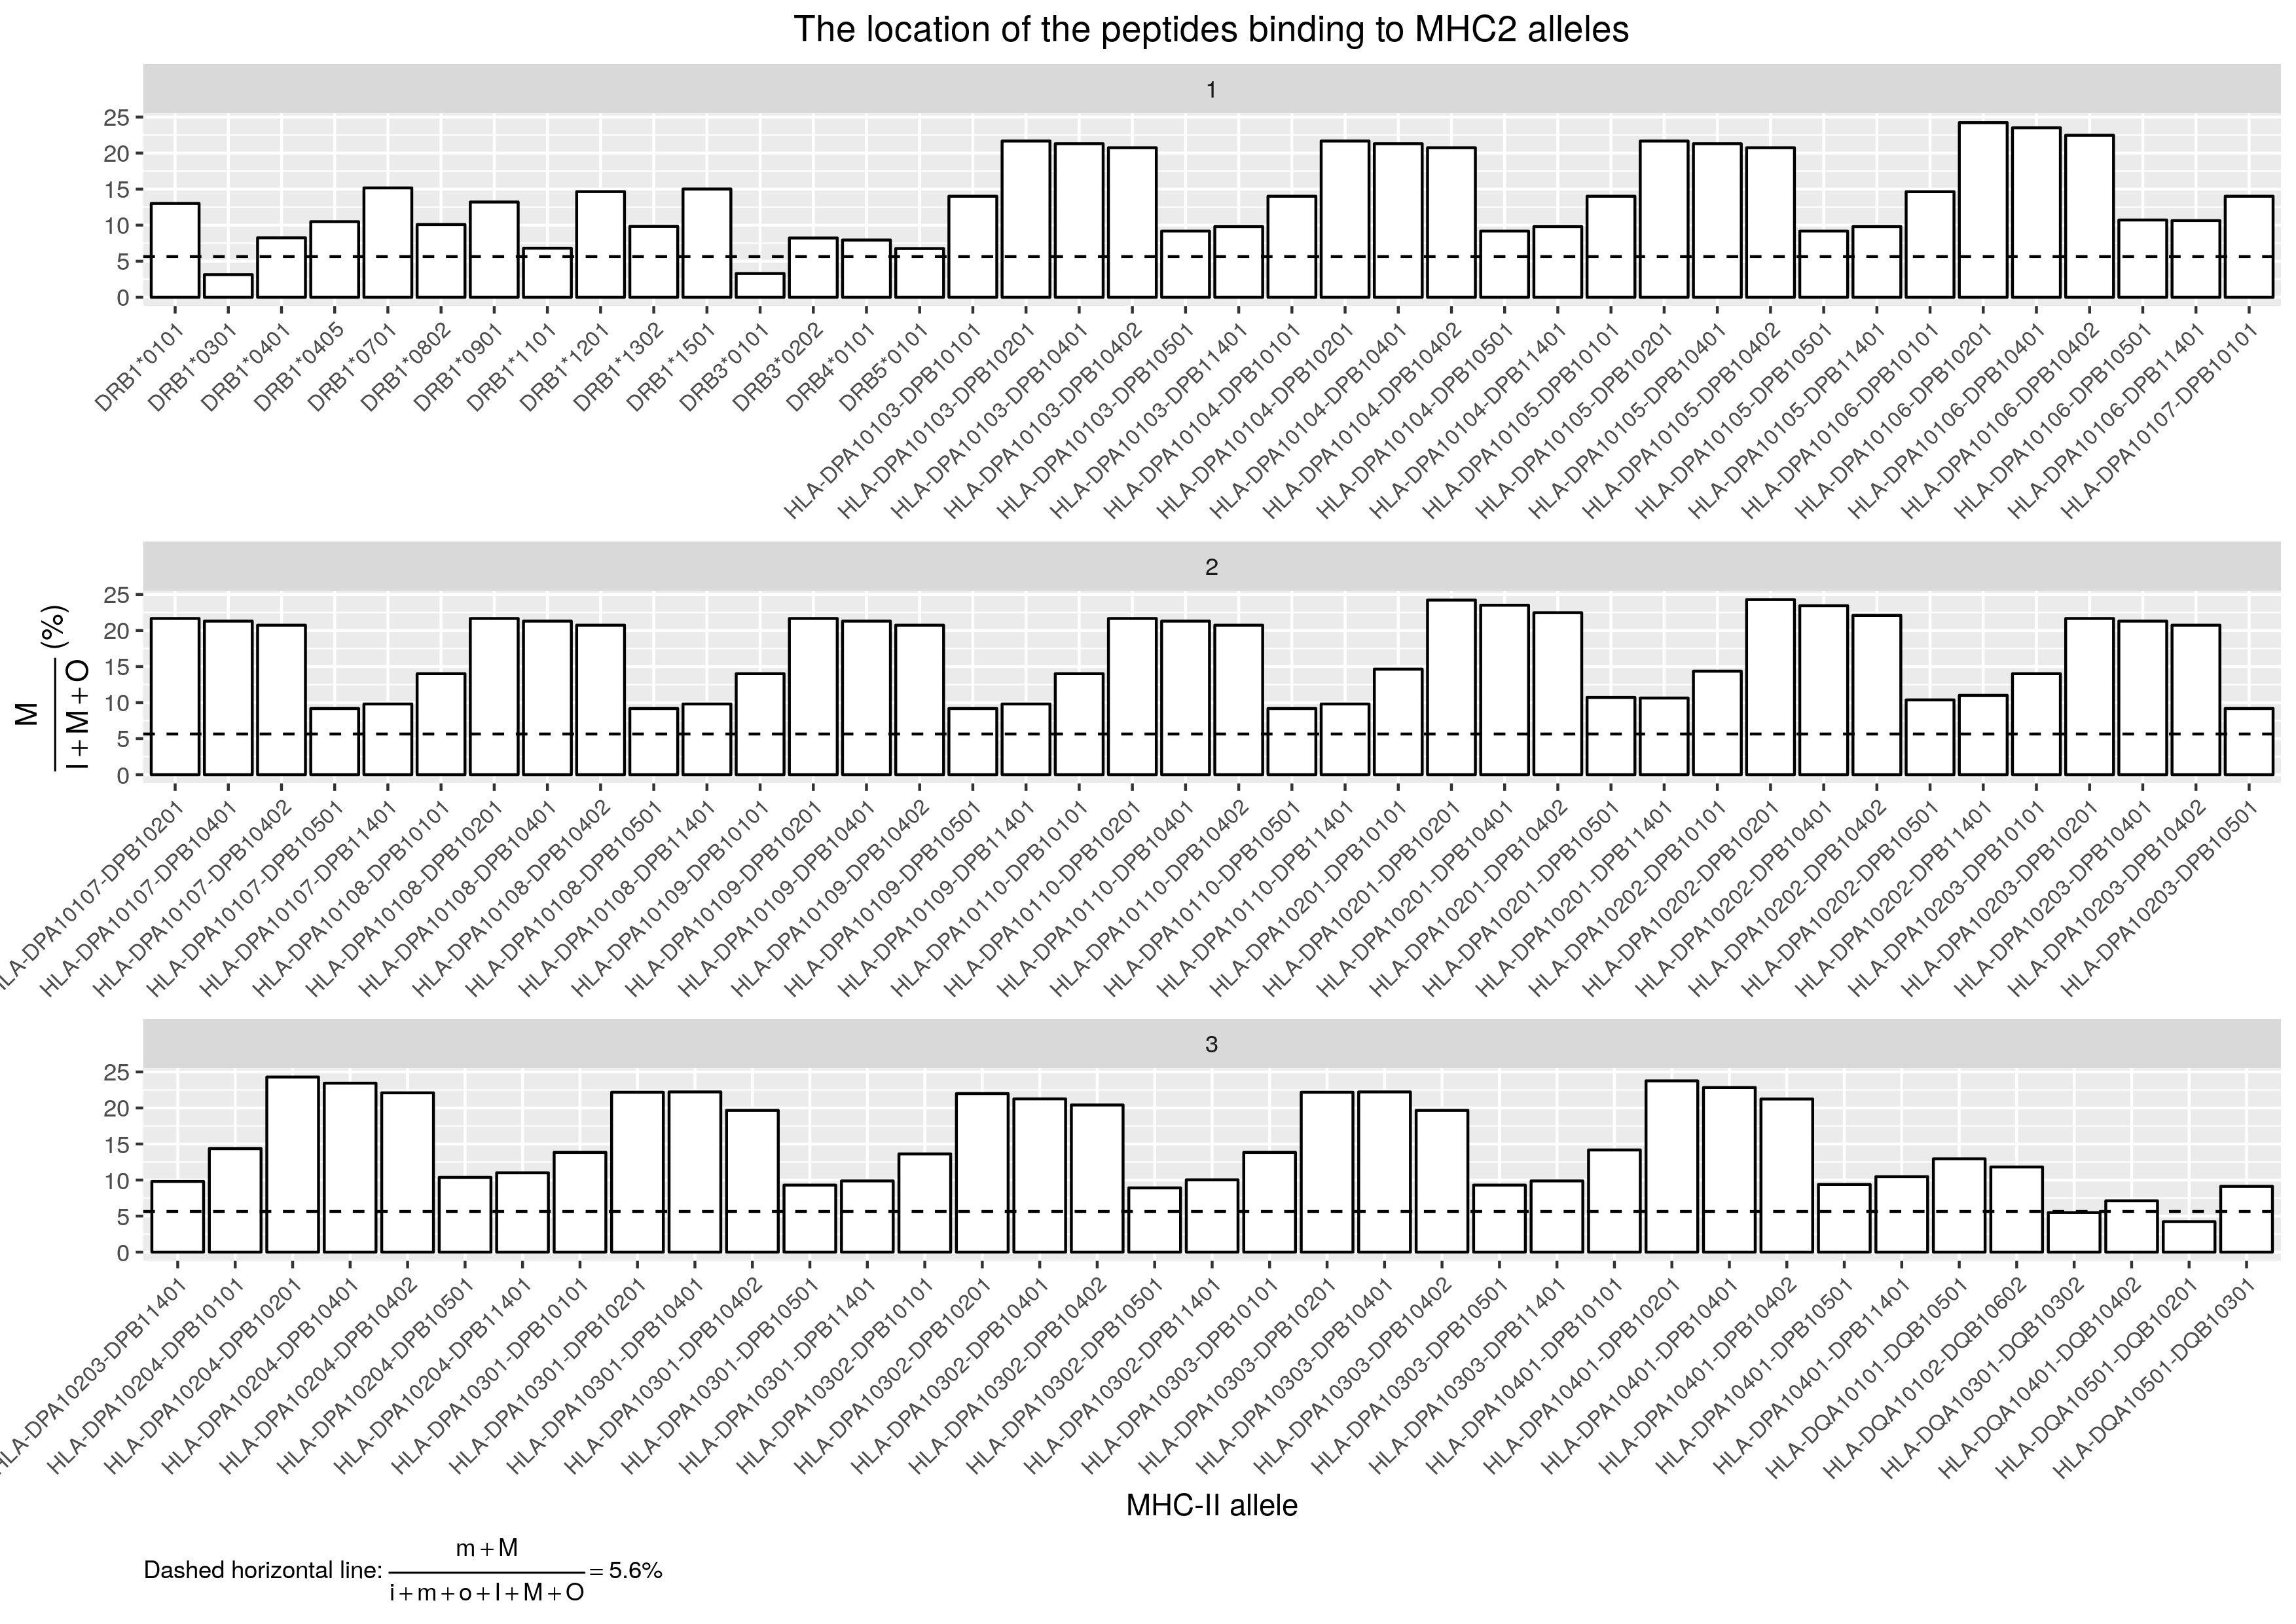
\includegraphics[width=\textwidth]{figure_1.png}
  \label{fig:1}
\end{figure}

\begin{figure}[ht]
  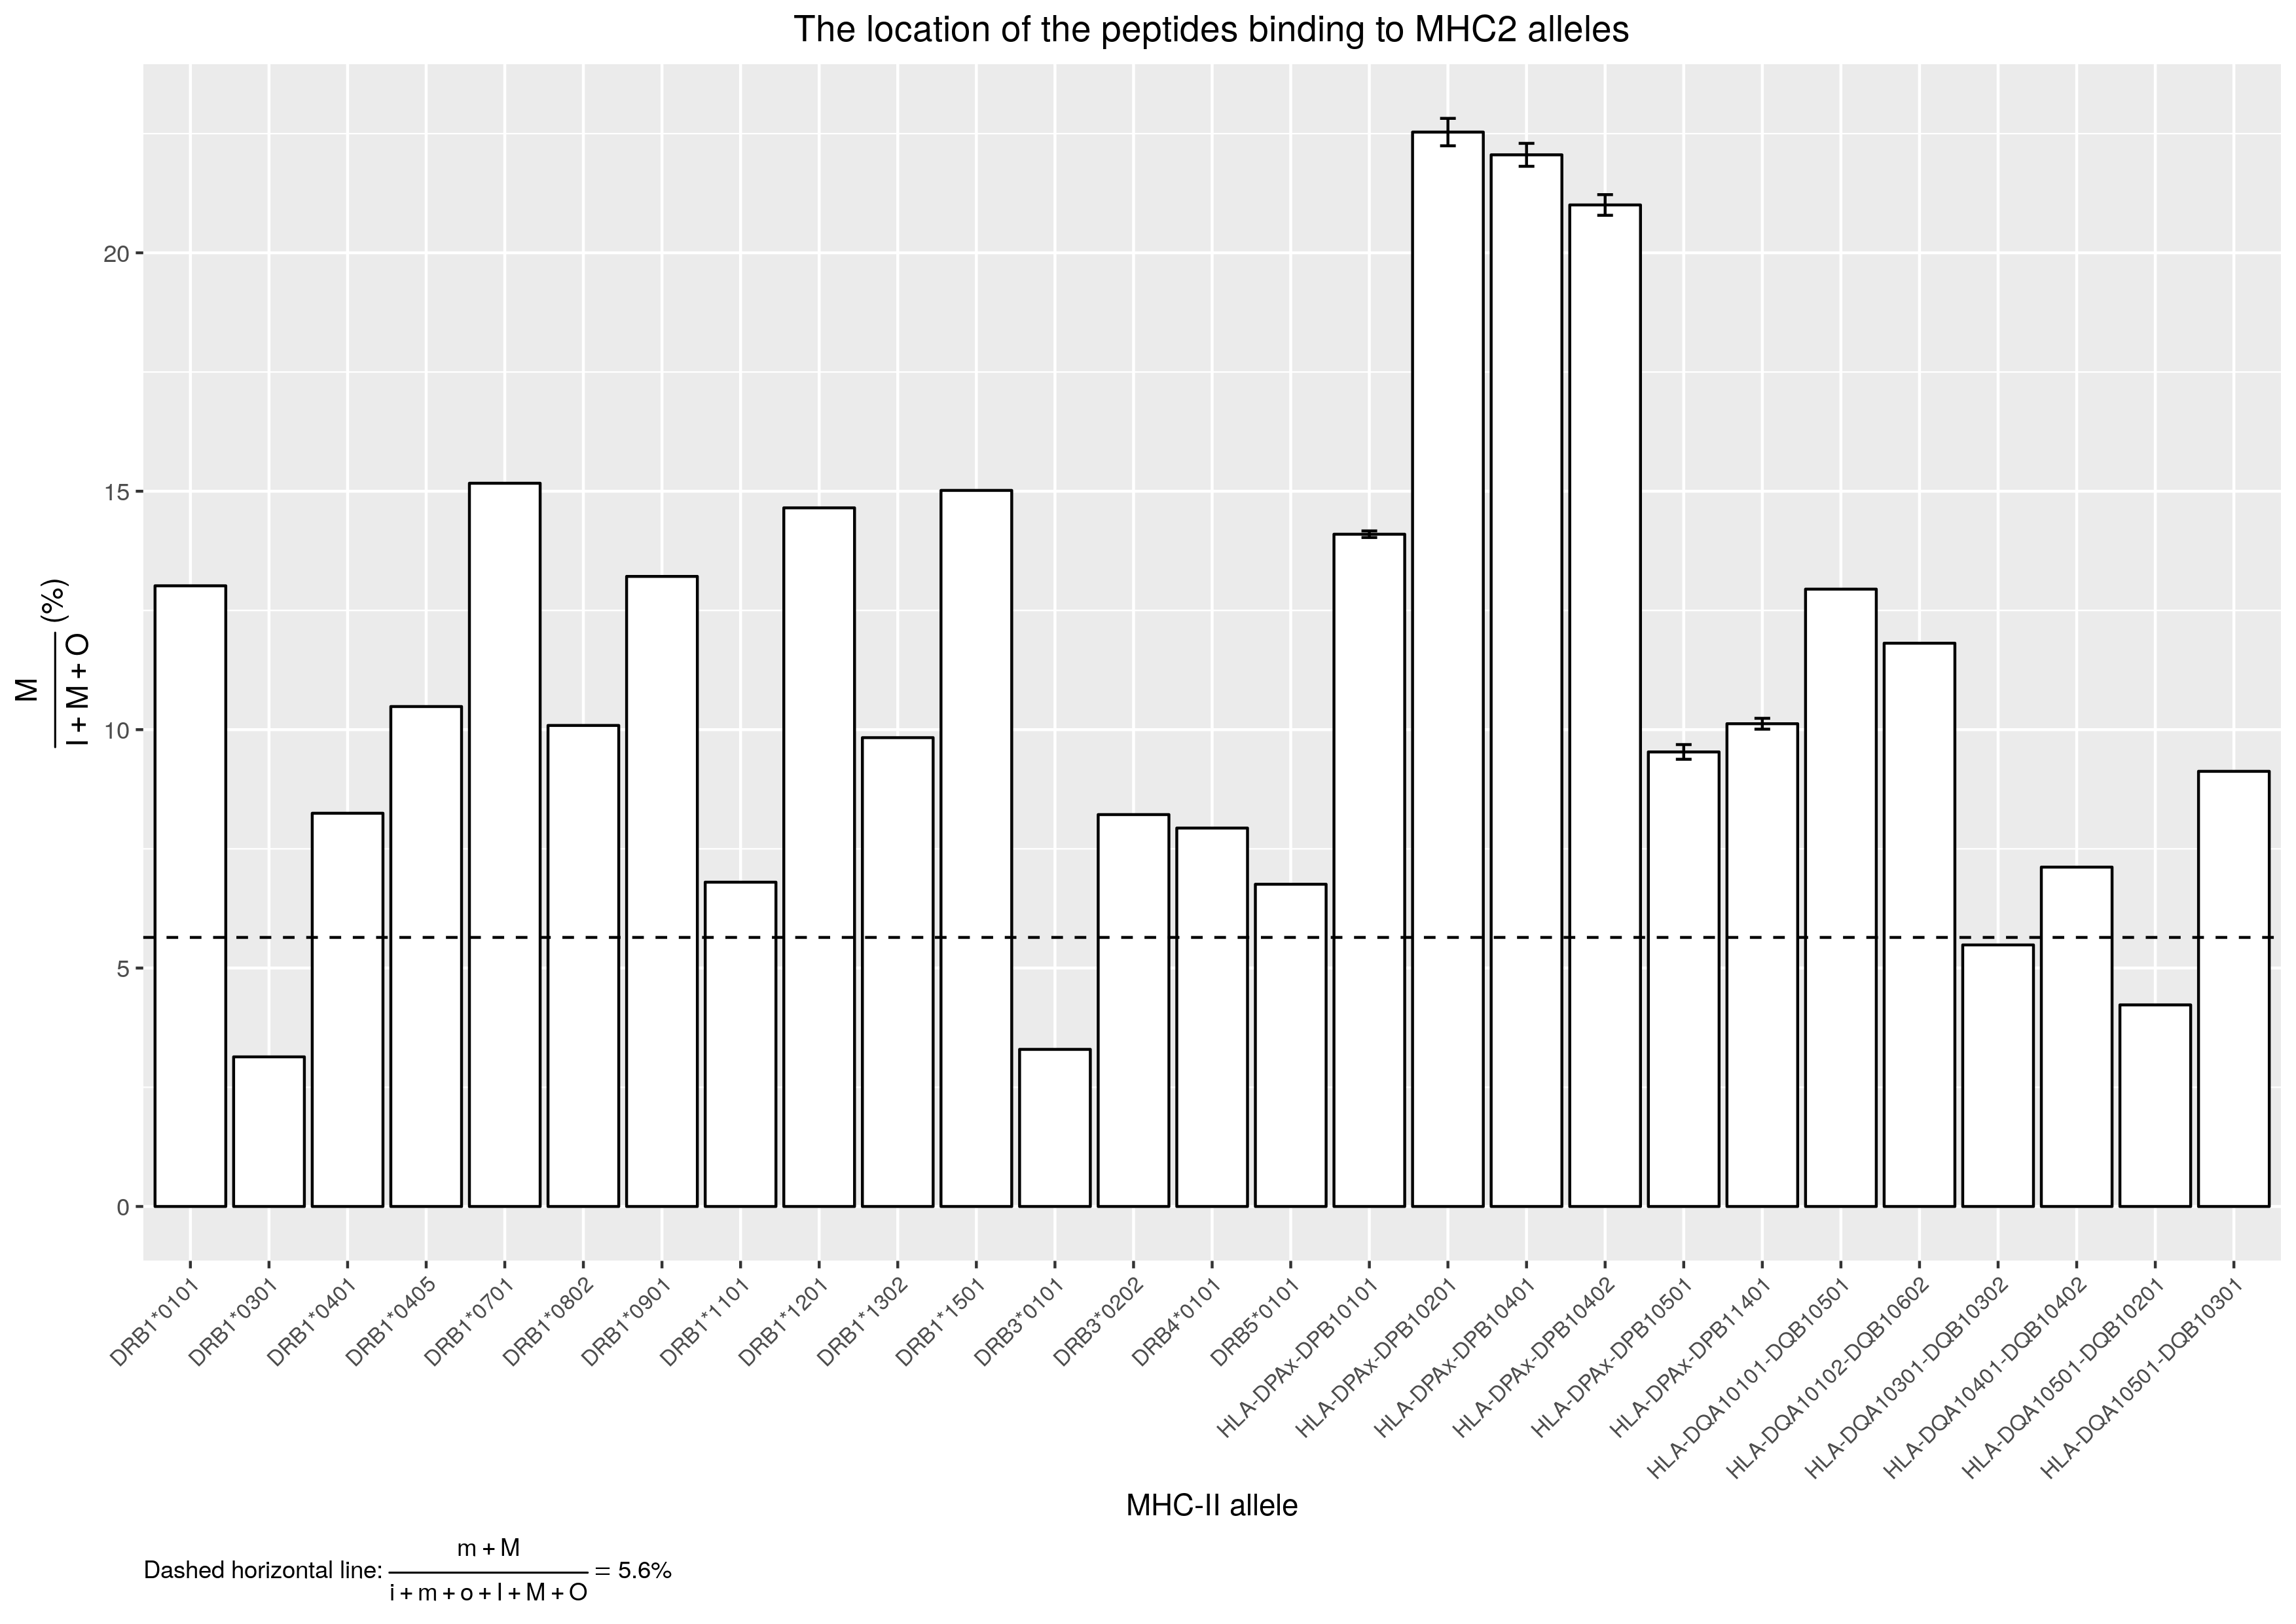
\includegraphics[width=\textwidth]{figure_1_5.png}
  \label{fig:1_5}
\end{figure}

\begin{figure}[ht]
  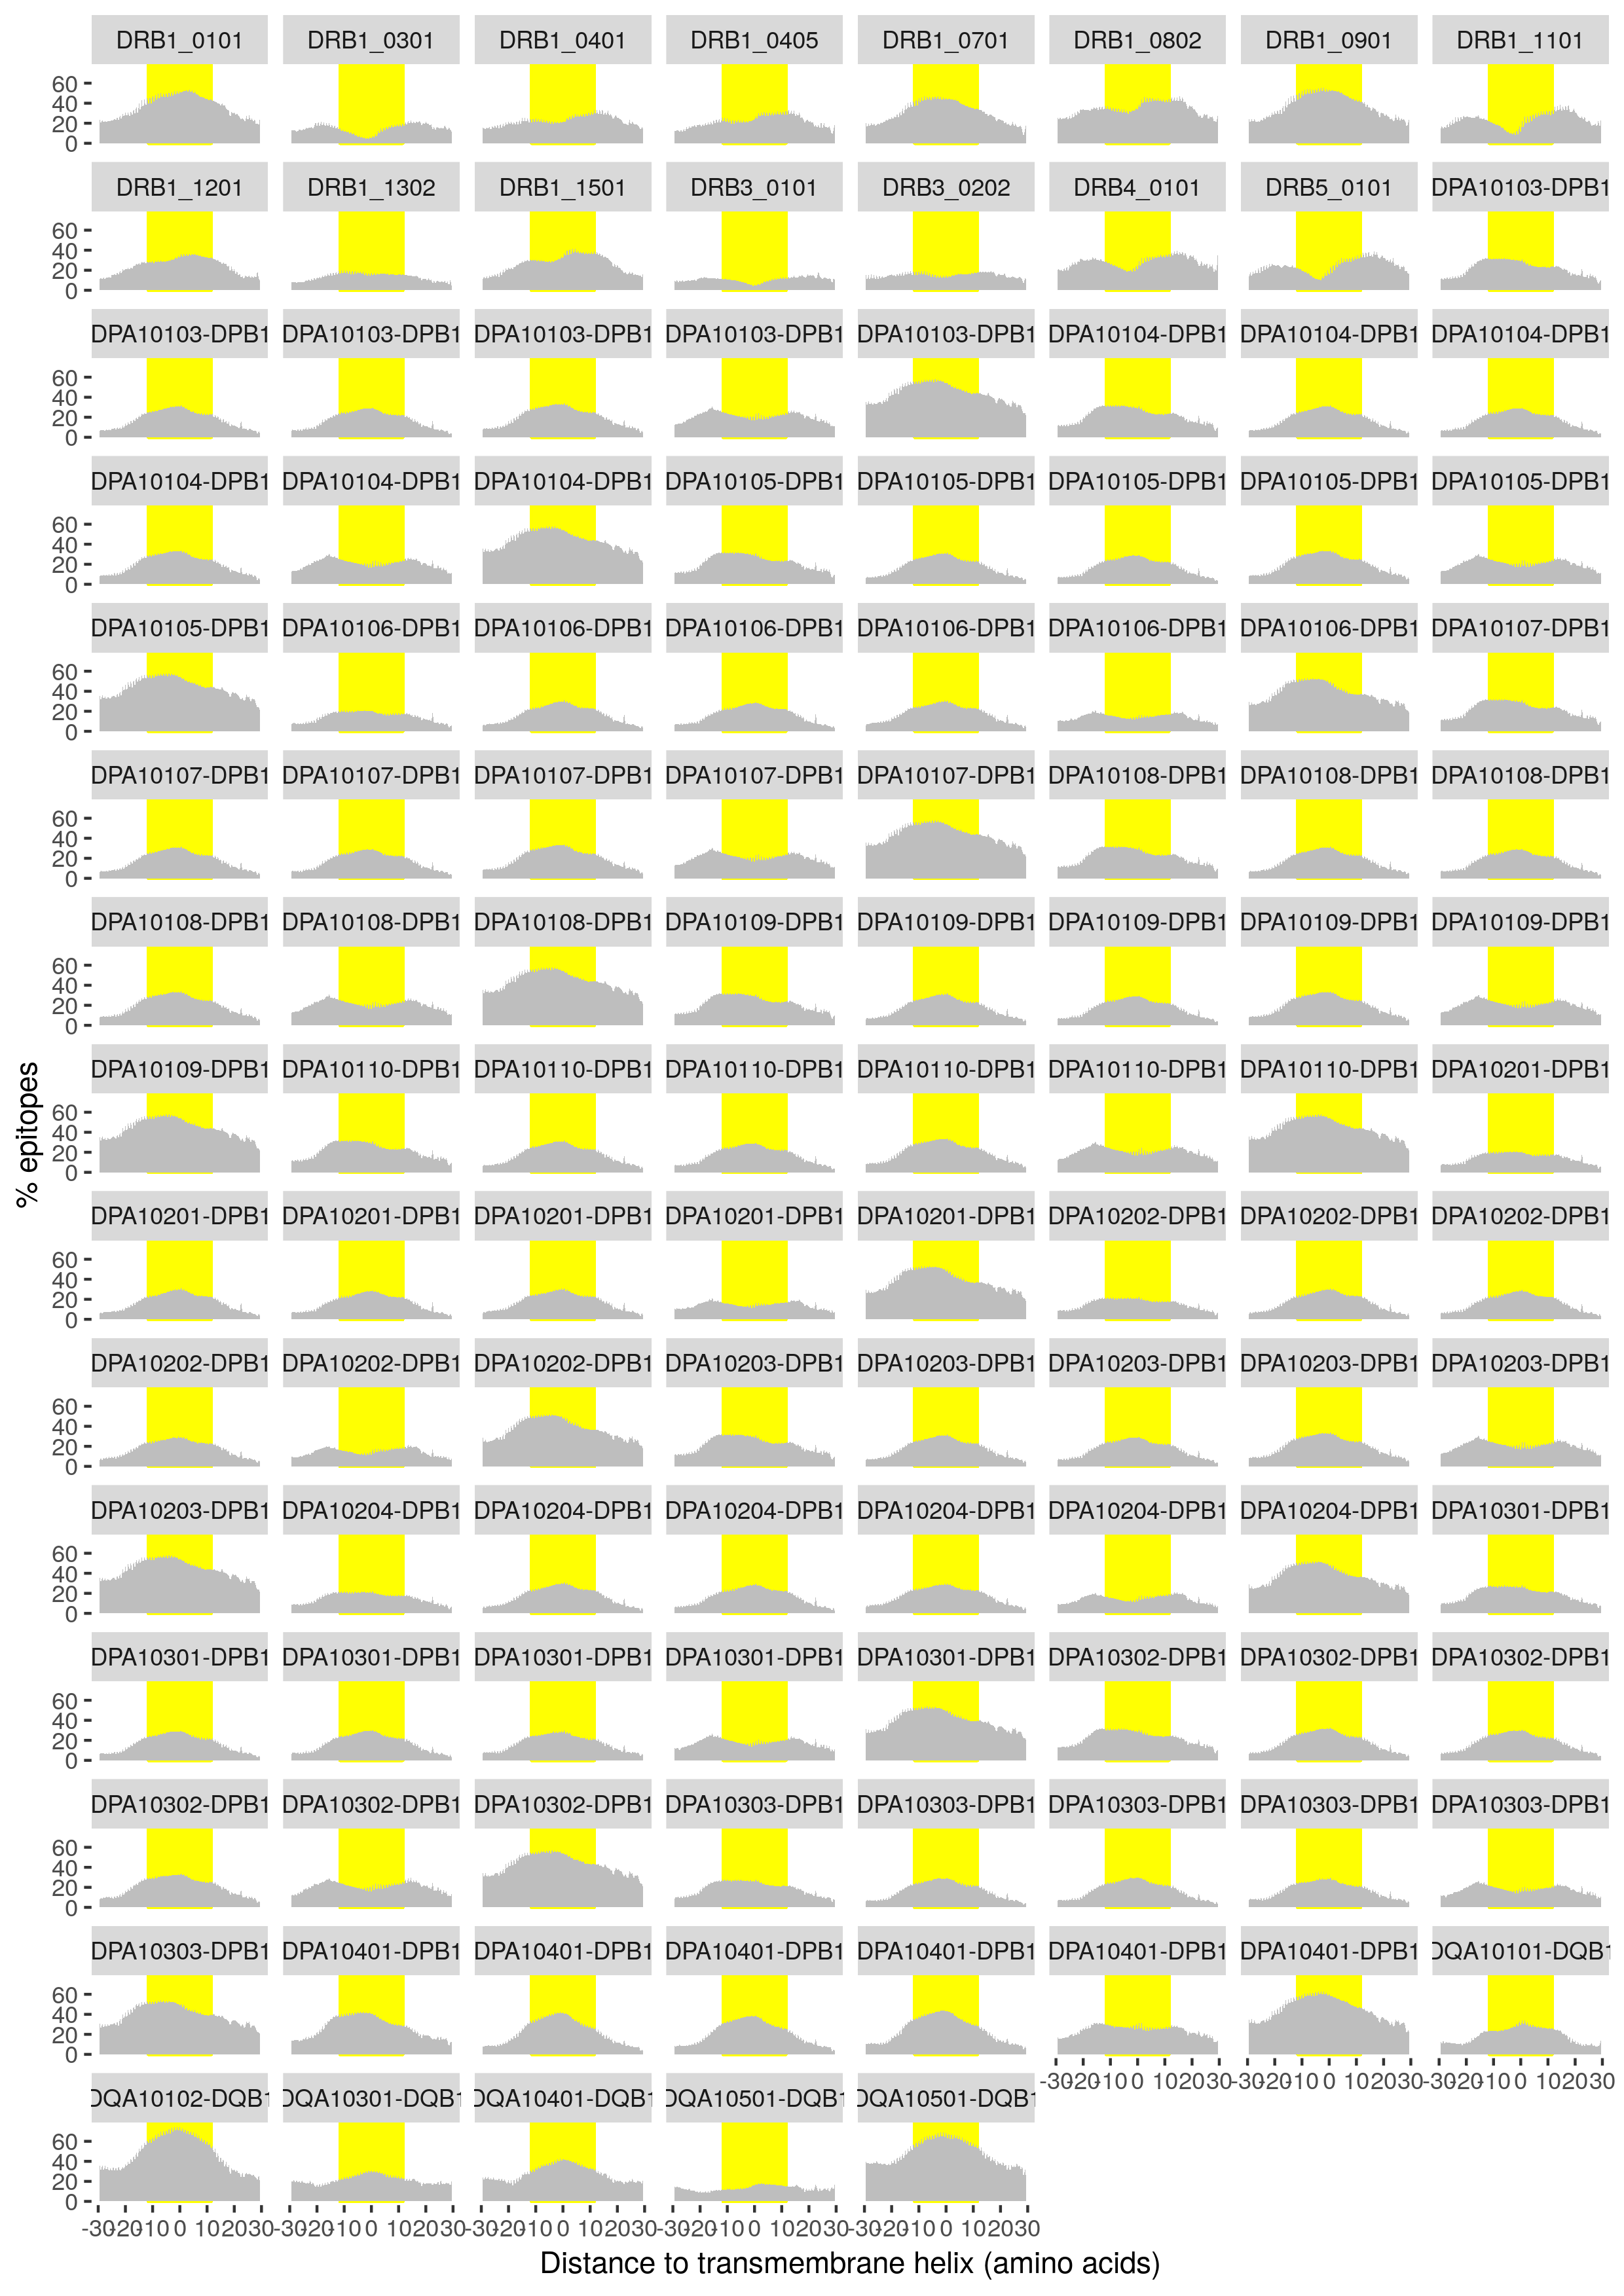
\includegraphics[width=\textwidth]{figure_3.png}
  \label{fig:3}
\end{figure}




\input{table_imoimo.latex}
% has label tab:results
\richel{
  I'd enjoy 
  (1) a row with 'expected by chance', 
  (2) using percentages instead,
  (3) merging inside and outside
}

The inference model with the highest evidence in the
TMH-only alignment was [yet unknown] and [also yet unknown]
for the non-TMH alignment. Individual model weights are shown
in tables \ref{tab:evidences_tmh} 
and \ref{tab:evidences_non_tmh}.

The Bayesian inference resulted in [a distribution of mutation rates],
as shown in [absent figure].
The ESSes of the Bayesian parameter estimates was above 200, exact values
are shown in tables \ref{tab:esses_tmh} and \ref{tab:esses_non_tmh}.

%%%%%%%%%%%%%%%%%%%%%%%%%%%%%%%%%%%%%%%%%%%%%%%%%%%%%%%%%%%%%%%%%%%%%%%%%%%%%%%%
\section{Conclusion}
%%%%%%%%%%%%%%%%%%%%%%%%%%%%%%%%%%%%%%%%%%%%%%%%%%%%%%%%%%%%%%%%%%%%%%%%%%%%%%%%

We conclude that MHC-II binds to TMH peptides with a higher/lower/equal
probability than expected by chance. 

We conclude that the evolutionary conservation if the TMH parts of membrane
proteins is higher/less/equal compare to its non-TMH counterparts.

%%%%%%%%%%%%%%%%%%%%%%%%%%%%%%%%%%%%%%%%%%%%%%%%%%%%%%%%%%%%%%%%%%%%%%%%%%%%%%%%
\section{Discussion}
%%%%%%%%%%%%%%%%%%%%%%%%%%%%%%%%%%%%%%%%%%%%%%%%%%%%%%%%%%%%%%%%%%%%%%%%%%%%%%%%

We compared the mutation rates between the TMH and non-TMH part of
multiple mycoplasma species. Where we expect no variation 
in mutation rate for every TMH amino acid,
\richel{
  we can test this, but unsure if that would make sense
}
we know that non-TMH part will have regions of different evolutionary
conservation: functional domains, especially in protein-protein
interactions will be strongly conserved, due to an even more constrained
set of peptides that enable a certain function.

\richel{
  Note that most bacteria are opportunistic pathogens.
  Note that most bacteria are generalists.
  Note that most bacteria have different cell membranes (and walls), that
  may have different functional constraints than a human cell membrane
}

%%%%%%%%%%%%%%%%%%%%%%%%%%%%%%%%%%%%%%%%%%%%%%%%%%%%%%%%%%%%%%%%%%%%%%%%%%%%%%%%
\section{Acknowledgements}
%%%%%%%%%%%%%%%%%%%%%%%%%%%%%%%%%%%%%%%%%%%%%%%%%%%%%%%%%%%%%%%%%%%%%%%%%%%%%%%%

We thanks to Geert van den Bogaart for his wisdom.

%%%%%%%%%%%%%%%%%%%%%%%%%%%%%%%%%%%%%%%%%%%%%%%%%%%%%%%%%%%%%%%%%%%%%%%%%%%%%%%%
\section{Data Accessibility}
%%%%%%%%%%%%%%%%%%%%%%%%%%%%%%%%%%%%%%%%%%%%%%%%%%%%%%%%%%%%%%%%%%%%%%%%%%%%%%%%

All code is archived at \url{http://github.com/richelbilderbeek/someplace},
with DOI \url{https://doi.org/12.3456/zenodo.1234567}.

%%%%%%%%%%%%%%%%%%%%%%%%%%%%%%%%%%%%%%%%%%%%%%%%%%%%%%%%%%%%%%%%%%%%%%%%%%%%%%%%
\section{Authors' contributions}
%%%%%%%%%%%%%%%%%%%%%%%%%%%%%%%%%%%%%%%%%%%%%%%%%%%%%%%%%%%%%%%%%%%%%%%%%%%%%%%%

RJCB and FB conceived the idea for this research. 
RJCB wrote the code.
RJCB and FB wrote the article.

%%%%%%%%%%%%%%%%%%%%%%%%%%%%%%%%%%%%%%%%%%%%%%%%%%%%%%%%%%%%%%%%%%%%%%%%%%%%%%%%
% Bibliography
%%%%%%%%%%%%%%%%%%%%%%%%%%%%%%%%%%%%%%%%%%%%%%%%%%%%%%%%%%%%%%%%%%%%%%%%%%%%%%%%
% MEE style
\bibliographystyle{mee}
\bibliography{article}
%%%%%%%%%%%%%%%%%%%%%%%%%%%%%%%%%%%%%%%%%%%%%%%%%%%%%%%%%%%%%%%%%%%%%%%%%%%%%%%%

\appendix

%%%%%%%%%%%%%%%%%%%%%%%%%%%%%%%%%%%%%%%%%%%%%%%%%%%%%%%%%%%%%%%%%%%%%%%%%%%%%%%%
\section{Model selection}
%%%%%%%%%%%%%%%%%%%%%%%%%%%%%%%%%%%%%%%%%%%%%%%%%%%%%%%%%%%%%%%%%%%%%%%%%%%%%%%%

\begin{table}[ht]
\centering
\begin{tabular}{rlllrr}
  \hline
 & Site model & Clock model & Tree prior & log(evidence) & Weight \\ 
  \hline
1 & JC & Strict & Yule & -8201.109 & 0.002 \\ 
  2 & JC & Strict & BD & -8203.346 & 0.000 \\ 
  3 & JC & Strict & CCP & -8195.927 & 0.278 \\ 
  4 & JC & Strict & CEP & -8194.976 & 0.720 \\ 
   \hline
\end{tabular}
\caption{
  Evidences for the TMH-only alignment
  \richel{These are just example values}
} 
\label{tab:evidences_tmh}
\end{table}

\begin{table}[ht]
\centering
\begin{tabular}{rlllrr}
  \hline
 & Site model & Clock model & Tree prior & log(evidence) & Weight \\ 
  \hline
1 & JC & Strict & Yule & -8201.109 & 0.002 \\ 
  2 & JC & Strict & BD & -8203.346 & 0.000 \\ 
  3 & JC & Strict & CCP & -8195.927 & 0.278 \\ 
  4 & JC & Strict & CEP & -8194.976 & 0.720 \\ 
   \hline
\end{tabular}
\caption{
  Evidences for the non-TMH alignment
  \richel{These are just example values}
} 
\label{tab:evidences_non_tmh}
\end{table}

%%%%%%%%%%%%%%%%%%%%%%%%%%%%%%%%%%%%%%%%%%%%%%%%%%%%%%%%%%%%%%%%%%%%%%%%%%%%%%%%
\section{Inference strength}
%%%%%%%%%%%%%%%%%%%%%%%%%%%%%%%%%%%%%%%%%%%%%%%%%%%%%%%%%%%%%%%%%%%%%%%%%%%%%%%%

\begin{table}[ht]
\centering
\begin{tabular}{rrrrrrrr}
  \hline
 & posterior & likelihood & prior & treeLikelihood & TreeHeight & YuleModel & 
birthRate \\ 
  \hline
1 & 10001 & 10001 & 10001 & 10001 & 9913 & 10001 & 9540 \\ 
   \hline
\end{tabular}
\caption{
  ESSes of the TMH-only alignment
  \richel{These are just example values}
} 
\label{tab:esses_tmh}
\end{table}

\begin{table}[ht]
\centering
\begin{tabular}{rrrrrrrr}
  \hline
 & posterior & likelihood & prior & treeLikelihood & TreeHeight & YuleModel & 
birthRate \\ 
  \hline
1 & 10001 & 10001 & 10001 & 10001 & 9913 & 10001 & 9540 \\ 
   \hline
\end{tabular}
\caption{
  ESSes of the non-TMH alignment
  \richel{These are just example values}
} 
\label{tab:esses_non_tmh}
\end{table}

\end{document}
